This section will discuss the feasibility of Artificial Neural Network as a technology for prediction of electricity prices and wind power. The hypothesis presented in Section~\ref{fig:sec:theHypothesis} and the experimental results will be the basis for discussions. Following quotation from the hypothesis section has been pointed out:

\begin{quotation}
\textit{Artificial Neural Networks can be characterised as Machine Learning\cite{18} and historical data that is relevant for the specific task will be used for training. The goal is to investigate and identify (through analysis and experiments) the importance of the influential factors to be included and represented in these datasets. Based on this we examine the feasibility of a Back Propagation Artificial Neural Network as a technology for predicting electricity prices and wind power.}
\end{quotation}

The hypothesis takes the outset in how to utilize the Artificial Neural Network best possible by analysing the influential factors, representing them appropriately and verifying it through experiments. Answering the feasibility question regarding ANN as a proper technology for predicting electricity price and wind power will be based on these parameters. It will be structured in the following way:

\begin{itemize}
\item Input analysis and transparency: This section will be dealing with the importance of investigating the influential factors.
\item Trustworthiness: The section considers the conducted experiments to verify the analysis and how to trust them.
\item Feasibility: Will conclude on the feasibility based on \#1, \#2 and our experimental results.
\end{itemize}

\subsubsection{Input analysis and transparency}
Artificial Neural Network as a technology for prediction in the electricity market is much dependent on the analysis and experiments surrounding it. The experiment discussions above highlight the need for analysing and documenting characteristics of what is to be predicted by the ANN. Machine Learning is data-driven\cite{18} and the analysis together with experiments point out the influential input parameters to include in the dataset that is the basis for the data-driven learning. The analysis will identify the input parameters to test and the experiments will either reject or verify what came out of the analysis. The result will be the best network setting along with a common understanding of exactly why these input parameters did the job for this market and why others did not. In continuation of this lies the need for transparency when using ANNs since omitting it will make it difficult to draw on the experience of others and make comparisons between systems due to the black box nature of the technology. Comparisons are of course possible if both attempted to predict the exact same market and used the exact same performance measure. Section~\ref{sec:inputParameterDiscussion} discuss the difference in experimental setups from publication to publication and how it becomes difficult to imitate when the information about it is incomplete. Based on discussions throughout the thesis and the comparison conducted in the experiment from Section~\ref{sec:priceExperimentThree} we argue that such comparisons isn't even fair due to the lack of documentation regarding input analysis, dataset and experiments. An example of a meaningful price parameter in the Danish electricity market which does not apply for all markets is wind speed due to the huge amount of wind mills in Denmark. This parameter shows a co-relation of 0,28 (Section~\ref{sec:Price}) and it is clear from the analysis why it has been included in the experiments where the influence is verified even to a greater extend than expected --- predicting the prices in a country without many wind mills should probably not expect the same benefits when using our setup with wind speed which should be apparent from the analysis in Section~\ref{sec:priceWeatherInfluence}. Another example exist for wind power where demand is analysed to greatly influence the production but is instead substituted with air density in the best prediction due to air density being calculated with temperature and pressure. Temperature highly influence demand and because pressure is close to constant the air density express temperature (see Section~\ref{sec:predictionBasicInputParams}). If not documented properly the use of these input parameters are unclear and it would require investigation and assumptions by others to replicate, and the overall benefits obtained in our experiments will most likely \emph{not} be the same when used in markets with different properties. It emphasizes what have been said earlier, namely that transparency in analysis is necessary to make comparisons and knowledge sharing possible but at the same time to identify the best possible setting yourself. The feasibility of the ANN should not be judged on its results alone (MAE, MAPE) but also on how and why the input parameters were selected and represented in the dataset. Both because what makes it applicable in one setting does not necessarily apply for another but also because we need to trust that the dataset (it is data-driven) is selected and tested based on a satisfactory foundation --- the resulting error can best be explained by looking at exactly what conditions constituted it. This leads to the trustworthiness of a system in terms of the experiments performed to verify the inputs which will be the topic of the next section.  

\todo{show the article that]}

\todo{include trimming}
\todo{we could have been more structured --> trend analysis and statistics}

\subsubsection{Trustworthiness}
A reliable prediction must have included all the right input parameters based on a comprehensive analysis in combination with a series of experiments that validate the findings. Section~\ref{sec:unseenDataDiscussion} emphasize and discuss the necessity of simulating predictions for at least a year to strengthen results. The year contains many different days and the seasons have different conditions, e.g. winter calls for heating and a lot of indoor activity whereas the summer is equal to holiday and being outdoor which is obviously reflected in the prices seen in Section~\ref{sec:seasonality}. The changes are also apparent for wind power but mostly due to the changes in weather conditions during the year (see Section~\ref{sec:windProdSeasonality}). The wind power seasonality is shown in graphs from section~\ref{sec:windPowerBestPredictionGraphs} where spring and fall have been highlighted here in Figure~\ref{fig:bestWPPredictSpringForDiscussion} and~\ref{fig:bestPredictWPFallForDiscussion} (the difference between the two should be apparent). We have shown examples of articles predicting only individual days or weeks and argue it to be sufficient (discussed in Section~\ref{sec:inputParameterDiscussion}). We consider it necessary to simulate whole years predictions for all experiments so that all conditional changes of every season are included and reflected in the results. Besides from the impact of different seasons our results showed a great variation in error according the starting point of the prediction. It emphasizes that different scenarios result in different results and must therefore be covered during testing. The discussion is elaborated in Section~\ref{sec:stepAheadForecastingDiscussion} where the potential elevated error depends highly on the starting point of the prediction. The trustworthiness of the prediction is related to from how many sides it has been seen and tests thereof to simulate the greater part of possible use cases. 

\begin{figure}[H]
\centering
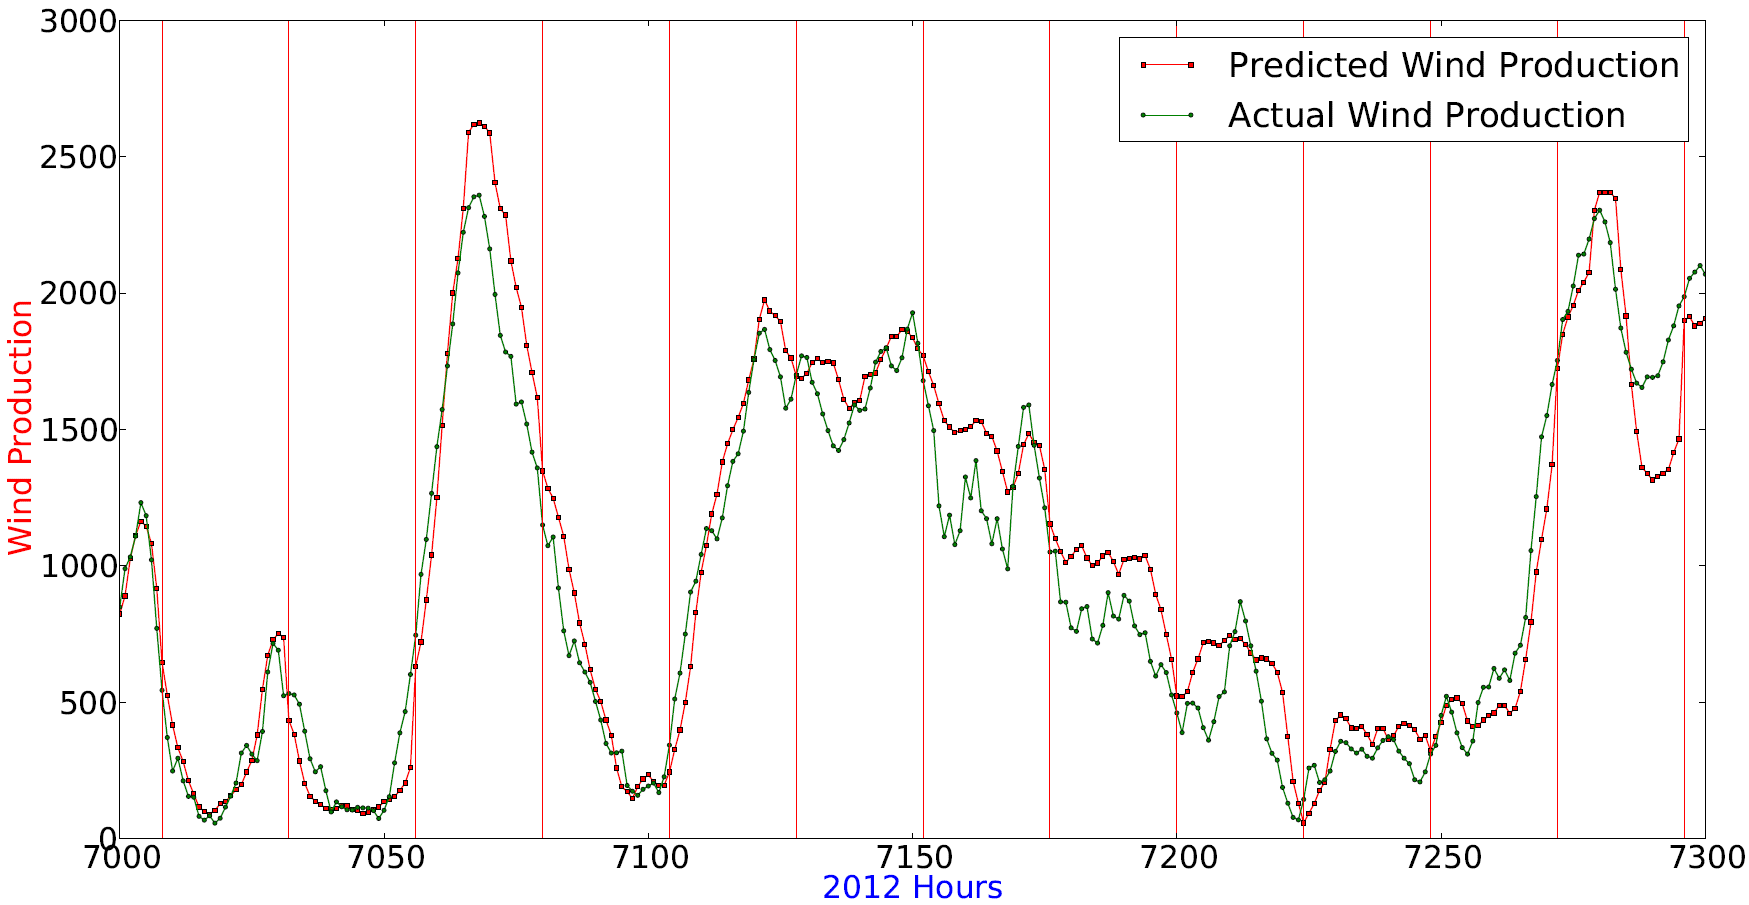
\includegraphics[width=0.99\linewidth]{billeder/bestPossiblePredictionWindProduction7000-7300_Fall.png}
\caption{Best prediction for 300 hours for Oct-Nov (Fall)}
\label{fig:bestPredictWPFallForDiscussion}
\end{figure}

\begin{figure}[H]
\centering
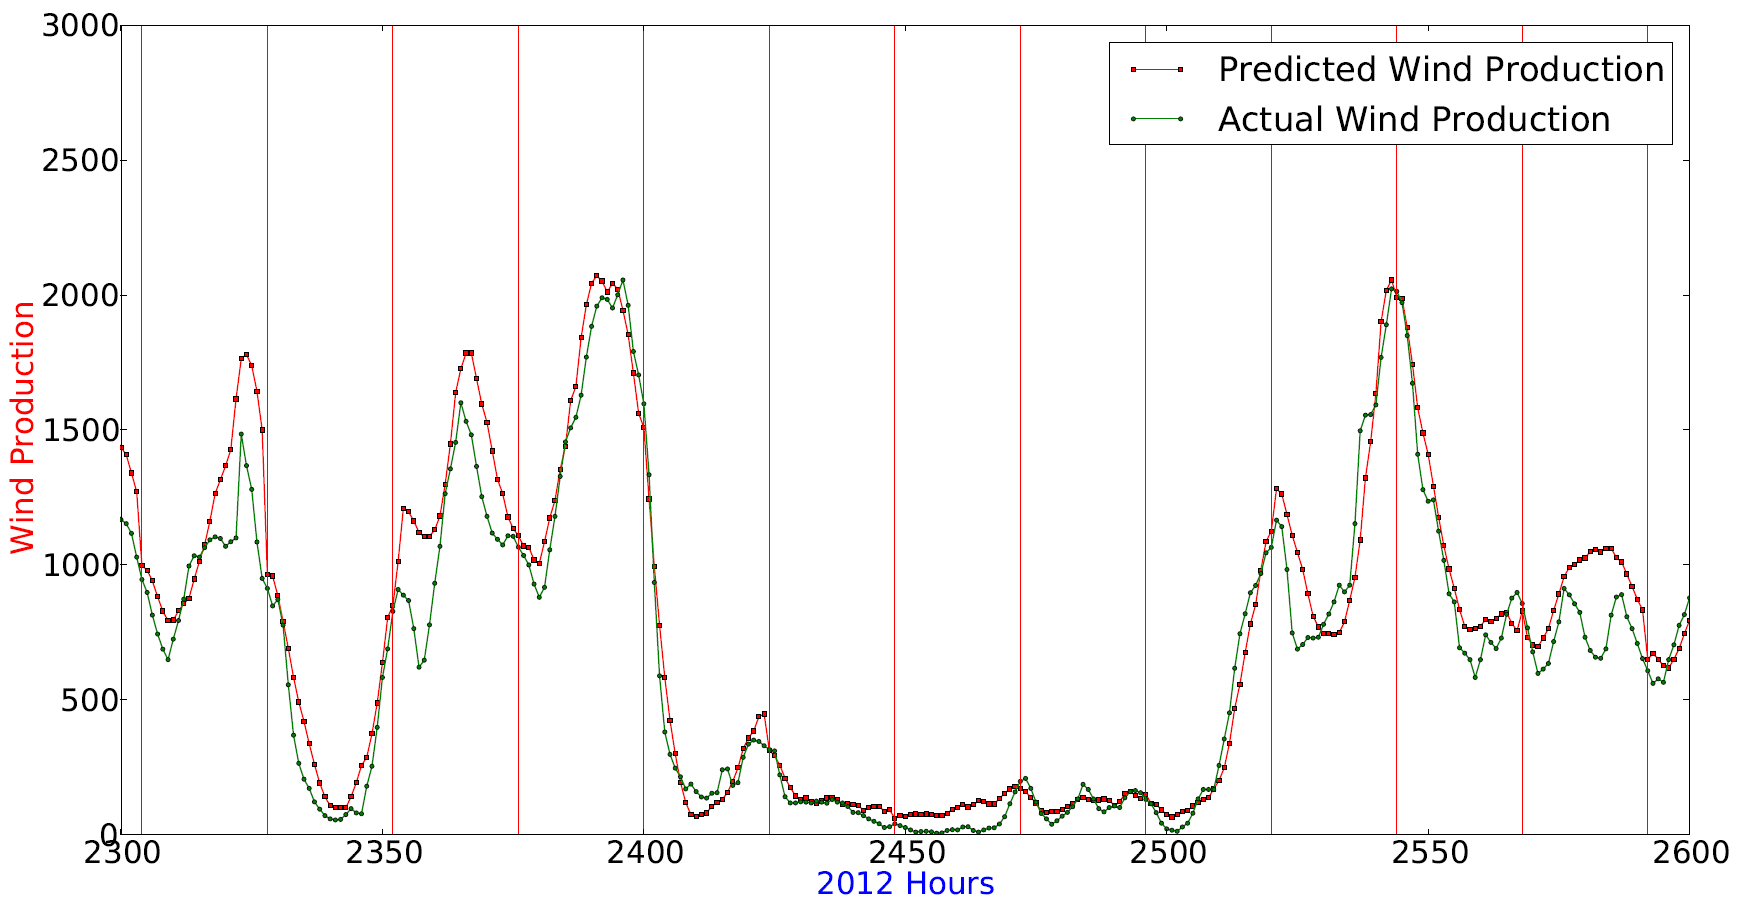
\includegraphics[width=0.99\linewidth]{billeder/bestPossiblePredictionWindProduction2300-2600_April_Spring.png}
\caption{Best prediction for 300 hours of April (Spring)}
\label{fig:bestWPPredictSpringForDiscussion}
\end{figure}

When arguing the need for testing on an entire year we must highlight the different results when running the same prediction again (discussed in detail in Section~\ref{sec:unseenDataDiscussion}. In our thesis we use an entire year to cover all conditions during a year as well as predicting similar days more than once. Another approach could be to run the yearly experiments more than once and deliver the average error for all test runs. This would strengthen the results bust must be a trade-off between time constraints and trying to cover most cases (exemplified in Section~\ref{sec:windPowerBestPredictionGraphs}). Another impact from our dataset could the fact that our testing set does not contain any predicted values. This can negatively affect the predictions when used in a real life setting and testing of this must be included in future work. We still consider the actual values to be sufficient since they look exactly the same and can simulate the predicted values in our experiments (simulation of a real setting). Furthermore, it gives us the opportunity to simulate all possible predictions on an entire year (since historical prediction data is not available) which our experiments show the importance of as described above. The analysis of the actual values show what influence the electricity price and wind power and in future work we must rely on other professionals to give us the best possible predictions of consumption and weather so that they are accurate enough to be consistent with the analysis. The weather predictions will deviate from the analysis \emph{only} if the they are inconsistent and inaccurate but as described in Section~\ref{sec:dataCollection} the accuracy of 24 hour weather prediction is 97\%. We consider the results obtained in this thesis valid because the potential decrease in accuracy would be applicable for all results, highly ranked or not. It correctly shows the co-relation between input/output, the ranking of results and the input combinations to be used. It must again be pointed out that the results are not definitive but indicate the influences of wind power and electricity prices as well as showing what data manipulations work for the Danish electricity market. The transparency of an Artificial Neural Network and its black box is considered a key to the feasibility of the predictions themselves because it implies trustworthiness. Transparency becomes of even greater importance when applying the ANN in a real life setting for decision making --- will be discussed in more detail later \todo{sec}.

\subsubsection{Feasibility}
The feasibility of the Artificial Neural Networks as a proper technology for prediction will be based on conclusions from the discussions just above and the experimental results as such. Results will not be compared to other Artificial Neural Networks since it has been found difficult and even unfair. Early discussions showed how comparison between ANNs require rebuilding and imitating of experimental setups and then running it on own datasets which in most cases is pointless due to different market conditions but at the same time difficult when documentation is incomplete. We made an example by attempting it in Section~\ref{sec:priceExperimentThree} where our own approach obtained 11\% better MAE than the other on our dataset. Without any prober analysis of their market, dataset and experimental setup we have no foundation for making any assumptions of their resulting error. We can conclude that with the information we were able to extract it did not work for the Danish electricity market. 

sec:influenceOfTrendInCalcInput

\todo{we have attempted to mimic and simulate real use which indicates that our modelled Artificial Neural Network can used in practice. }

One article \cite{forecastingSpotPricesAccountingForWindPower} forecasts the Danish spot prices from nord pool spot which is the exact same prices used in this thesis. They use instead a time-varying regression model and more sophisticased two-step models to 

To sum up the conclusions of the last two sections:

\begin{itemize}
\item The feasibility of the proposed ANN can be seen as a direct result of the identified inputs parameters and their representation. The analysis, the actual selection of inputs and the experiments is what constitutes the prediction and explains the obtained experimental results --- it is also what creates trustworthiness in the results (MAE, MAPE). The prediction is data-driven and no better than the dataset its trains upon. The feasibility should therefore be mentioned based on the analysis of input parameters and how they were validated through experiments. This of course presupposes that the prediction experiments must cover as many scenarios as possible. Days are different and the overall feasibility of the ANN is not conveyed if not tested on a satisfactory amount of data. We argue that the final prediction error cannot stand alone without a description of exactly what constituted it and why.
\end{itemize}

We have satisfied the above by a thorough analysis of the influential factors for electricity price and wind power for the Danish electricity market in Chapter~\ref{ch:theANNs} which have been validated through various experiments performed on an entire year in Chapter~\ref{ch:experimentalResults}. The experimental results show how the predictions evolve from experiment to experiment and how the different strategies affect the prediction results. To rationalise the feasibility of the system in terms of our actual results we will highlight the best prediction from both price and wind power.

\begin{itemize}
\item The best prediction showed the most influential parameters for out experimental setup to be wind speed, temperature, last known wind power, time of day and historical volatility. Wind power follows wind power, temperature substitutes demand,
\end{itemize}
 

\todo{dss will be followed by the conclusion: the accuracy requirement much depends on use cases}

\todo{discuss results and show graph}

\todo{just a number if you can't compare it anything due to the different markets} 

\todo{to our knowledge nobody have tried what we have with wind prod}

(grease the wheels)


\todo{vi mener ligeledes ikke at man kan sammenligne disse ting --- first of all it requires the same setup but also differences on markets plays in}


Vi kan ikke direkte sammenligne uden at imitate og det er ikke meningen med dette speciale.

\todo{Det kan helt sikkert bruges til at forudsige. Vi kan se trend, vi kan se at vi curve fitter. Det er en anden diskussion, hvis vi inkluderer specifikke brugsscenarier, da kraever helt konkrete eksempler paa brug og hvad der oenskes opnaaet}

\todo{The best result missed its target (in average) by 121 out of the interval from 0 to 2753 corresponding to 4,4\% of the 2753 potential values -- wind power. 7,9 \% for price, 45,11 out of interval from 61 to 632 = 571}

\subsubsection{Potential improvements}



\todo{initialization of random weights === different results ... should train more for better results, but they only test 10 weeks. --> adaptive forecasting}

\todo{adaptive forecasting --- use weights that worked last time instead of initial randomization}

Trimming\todo{section}

\todo{have we tested enough --- the time it takes to do all testing. You need to be smaaart --- use intuition}

TODO: talk about how testing is time consuming. All tests run for long time

TODO: the results are not definitive but what we can do is see tendencies in what parameters really matter.

TODO: ideal world endless test --> neural network requires a lot of testing

The above discussions comply well with the fact that machine learning is not all technical bot also intuition, creativity and black art\cite{18}. For instance a great deal of intuition and creativity goes into designing the experiments. Everything cannot be tested and you must rely on intuition to include the all situations necessary for testing, and the creativity resides in how to actually do it. Furthermore, the different inputs can be represented in various ways that calls for creativity --- represent input as a matrix, calculate slope or volatility and represent the seasonal aspect as month or summer/winter/spring/fall. The ANN being black art or a black box requires intuition in itself since we cannot foresee the outcome. When analysing prediction results from the experiments we rely on the analysis but also our intuition, especially in cases where things are not as expected. We must assume based on the analysis and our intuition that this was what happened. It is again an argument for analysis and experiments to be documented for both yourself and the sake of transparency.





\todo{black art --> different results on same data every time. Don't know how the relationship is found}


\todo{mae vs. mape. Mape is used because it makes it easier to compare.. cite yamin2004adaptive}


Of course networks is much more --- black box. trial error.



An Artificial Neural Network is as good as the underlying data. 



Neural works as basis for a decision support system. If ANN can predict can it then be used in the real life? Discussion about how this is related the text where the results are ambiguous 
Artificial Neural Networks can it itself be considered as a Optimization Based Support Model which is described in Section \todo{section and discuss further}. The trust of the forecast is critical and especially when dealing with ANNs because they are a black box. 

Discuss this in relation to DSS and how it relates to it. It is here important to emphasize that in order to use this a lot of things around it has to be build. When used in a real life setting the user just need to know the input, a high level description of what happens and then the output.
This is not a one-click solution and it requires a lot of configuration \todo{vi har masser skrevet om dette, ref, trade-offs, small / big values. Step-ahead forecasting, trimming, size}. The system is for experts and they can base there prediction on there own experience --- for instance an expert might now that high prices now together with the current market won't most likely won't result in lower prices, therefore the system does not need to consider low values. High configurable but still easy-to-use.

